\chapter{Future Work} \label{fw}

The future work for this PhD will look at different techniques to finding stopping points. Specifically we will focus on text processing approaches to stopping.



Any area that could be further expanded on is the use of using the similarity score in the initial rankings as a basis for comparing documents. In novel work section \ref{simScoreMethod} we examined a technique that uses the top document as the origin point for comparing subsequent documents. To improve the accuracy of the origin point we could try using different points and taking average over a set of points:


\begin{figure}[H]
\center
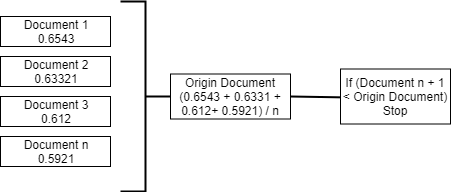
\includegraphics[height=4cm]{figures/originMethod.png}
\caption{Calculating Origin Average}
\end{figure}

The \% difference between document $n+1$ and the origin document would still be used to derive the stopping point.

This approach has the advantage of taking into consideration variability in the quality of the rankings. It also has the advantage of being entirely unsupervised and does not require us to sample the initial document collection. 

A further development of this method is to create an origin document using the document text content itself:

\begin{figure}[H]
\center
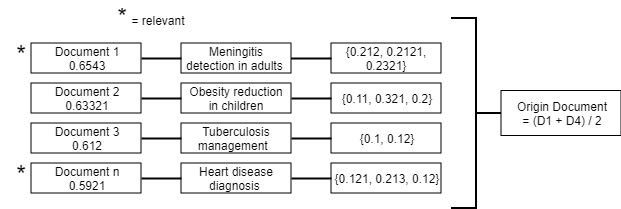
\includegraphics[height=4cm]{figures/origin2.png}
\caption{Generating Origin vector using document content}
\end{figure}

Here we have a further development in that we are using the top $n$ documents to calculate a average a document vector by using the content of the document. We can then use vector similarity comparisons such as euclidean distance and cosine similarity to compare the origin document vector to further documents down the rankings.



\section{Gnatt Chart}

\begin{sidewaysfigure}


\begin{figure}[H]
\center
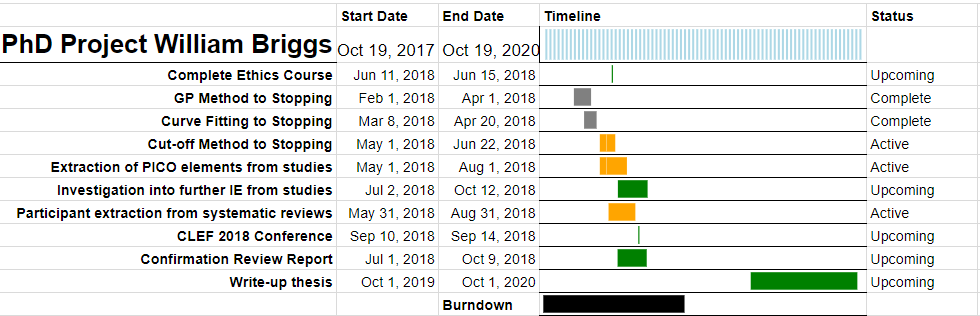
\includegraphics[height=7cm]{figures/gnatt.png}
\caption{Gnatt Chart}
\end{figure}
\end{sidewaysfigure}


